% =============================================================================
% Section 6 — Comparaison transverse et transfert des méthodes
% À insérer juste avant la conclusion du rapport.
%
% Pré-requis :
%   \usepackage{booktabs, graphicx, float, amsmath, amssymb, hyperref}
%
% Figures et tableaux référencés (à placer dans figures/ ou à adapter) :
%   - figures/cross_auc_heatmap.pdf
%   - statap_code/cross_dataset/data/cross_table.tex (optionnel : pivot complet)
% =============================================================================

\section{Comparaison transverse et transfert des méthodes}
\label{sec:transverse}

\subsection{Motivation et protocole}

Les sections précédentes ont chacune étudié un couple
particulier (méthode, dataset)~: la prédiction conforme sur MMLU, le
lien confiance--vérité sur des questions numériques courtes
(section~\ref{sec:confiance_verite}), l'analyse des log-probabilités
sur des générations longues (section~\ref{sec:generations_longues}), et
WEPR sur la version textuelle de TriviaQA (section~\ref{sec:wepr}). Cette structure permet une
analyse fine de chaque cadre, mais ne dit rien de la robustesse des
méthodes lorsqu'on les applique à un dataset pour lequel elles n'ont
pas été conçues. Or c'est précisément ce point qui détermine leur
utilité pratique : un score d'incertitude n'est utile que s'il garde sa
capacité de discrimination quand on change le type de tâche, la
longueur des générations ou le régime de prévalence des erreurs.

Cette section construit ce dialogue. Trois ponts sont établis. Premièrement,
le modèle WEPR introduit en section~\ref{sec:wepr} est entraîné et évalué
sur les générations Chain-of-Thought de GSM8K (cadre de la
section~\ref{sec:generations_longues}), ce qui permet à la fois une
comparaison directe à la régression à 64~variables de cette même
section et une mesure du transfert inter-domaines. Deuxièmement,
l'\emph{entropie sémantique} (Kuhn et al., 2023), que nous avions
implémentée sur ELI5, est appliquée au cadre numérique de la
section~\ref{sec:confiance_verite} afin de mesurer ce qu'elle apporte
au-delà des log-probabilités internes. Troisièmement, une table croisée scores~$\times$~datasets est
construite pour synthétiser visuellement les trois sections du rapport
en un seul objet.

\subsection{WEPR sur GSM8K et transferts inter-domaines}
\label{sec:transfert_wepr}

\paragraph{Régénération du dataset.}
La section~\ref{sec:generations_longues} a entraîné une régression
logistique à 64~variables dérivées des log-probabilités sur~1\,319
réponses GSM8K générées avec un raisonnement détaillé, atteignant une
AUC de~0,729. Pour comparer cette approche à WEPR, nous régénérons les
réponses sur les mêmes questions GSM8K avec~$K=10$~candidats top-K
stockés à chaque position, en utilisant un prompt qui demande
explicitement un raisonnement étape par étape suivi de la réponse
numérique au format JSON. Le modèle (Gemini~2.0 Flash, $T=1{,}0$)
atteint une exactitude de~96{,}1\% sur les~1\,319 questions, ce qui
correspond à un déséquilibre marqué (1\,268 réponses correctes
contre~51 incorrectes).

\paragraph{Trois sous-séquences pour localiser le signal.}
Chaque génération est ensuite découpée en trois sous-séquences~:
l'ensemble des tokens (\emph{full}), les tokens du raisonnement seul
(\emph{reasoning}), et les tokens de la réponse numérique finale
(\emph{answer}). Le modèle WEPR à $2K=20$~variables est entraîné
séparément sur chacune de ces trois sous-séquences (validation croisée
à 5~plis stratifiés). Les résultats sont reportés dans le
tableau~\ref{tab:wepr_gsm_subseq}.

\begin{table}[H]
\centering
\caption{WEPR entraîné sur GSM8K — performance par sous-séquence.
AUC en validation croisée à~5~plis. EPR désigne la baseline non
supervisée (entropie tronquée moyenne) sur la même sous-séquence.}
\label{tab:wepr_gsm_subseq}
\begin{tabular}{lccc}
\toprule
Sous-séquence & Tokens (moy.) & AUC WEPR (CV) & AUC EPR \\
\midrule
Full      & 188 & $0{,}726 \pm 0{,}149$ & 0{,}814 \\
Reasoning & 180 & $0{,}717 \pm 0{,}156$ & 0{,}811 \\
Answer    &   8 & $0{,}571 \pm 0{,}080$ & 0{,}640 \\
\bottomrule
\end{tabular}
\end{table}

Trois enseignements ressortent. Tout d'abord, WEPR appliqué à la
\emph{full generation} obtient une AUC en validation croisée de~0{,}726,
indiscernable de la valeur de~0{,}729 reportée dans la
section~\ref{sec:generations_longues} avec une régression à~64 variables. Cette
égalité est obtenue avec une représentation trois fois plus
parcimonieuse, ce qui suggère que la richesse de la collection de
features manuelles utilisée en section~\ref{sec:generations_longues}
ne fait que recapturer ce que la structure top-K encode déjà. Ensuite, l'écart entre
\emph{reasoning} (0{,}717) et \emph{answer} (0{,}571) confirme avec
WEPR ce que la section~\ref{sec:generations_longues} avait observé sur les variables
manuelles~: le signal d'erreur réside dans le raisonnement, pas dans la
conclusion. Enfin, la baseline EPR donne ici 0{,}81 sur les
générations complètes — un niveau étonnamment élevé, supérieur même à
WEPR sur cette sous-séquence prise seule (la différence n'est cependant
pas significative compte tenu de l'écart-type de WEPR à~0{,}15, lié au
faible effectif de la classe minoritaire). Cela indique que sur
GSM8K, l'entropie tronquée moyenne contient à elle seule l'essentiel de
l'information utilisable, et que la pondération apprise par WEPR ne
change l'ordre que marginalement.

\paragraph{Transfert TriviaQA $\leftrightarrow$ GSM8K.}
Pour évaluer le degré de spécificité de WEPR à un dataset, nous
appliquons le modèle WEPR entraîné sur~73\,793 questions TriviaQA
(section~\ref{sec:wepr}) aux générations GSM8K, et inversement. Le
tableau~\ref{tab:transfer_wepr} présente la matrice~$2 \times 2$
résultante.

\begin{table}[H]
\centering
\caption{Transfert de WEPR — AUC selon le couple
(modèle, dataset d'évaluation). Les valeurs diagonales sont les
performances en domaine d'entraînement.}
\label{tab:transfer_wepr}
\begin{tabular}{lcc}
\toprule
                              & \'Eval.\ sur TriviaQA & \'Eval.\ sur GSM8K \\
\midrule
Modèle TriviaQA               & \textbf{0{,}681} (in-domain) & 0{,}793 (transfert) \\
Modèle GSM8K                  & 0{,}477 (transfert)          & \textbf{0{,}829} (in-domain) \\
\bottomrule
\end{tabular}
\end{table}

Le résultat le plus saillant est l'asymétrie complète du transfert. Le
modèle TriviaQA, appliqué tel quel à GSM8K, obtient~0{,}793 — soit une
AUC \emph{supérieure à sa performance en domaine d'origine}~(0{,}681).
Ce résultat est moins paradoxal qu'il n'y paraît. Le déséquilibre
extrême de GSM8K (96\% de réponses correctes) gonfle mécaniquement
l'AUC, et les coefficients de WEPR-TriviaQA sont stables et de faible
amplitude, encodant un signal générique d'instabilité distributionnelle
qui se transfère bien à un cadre adjacent. À l'inverse, le modèle
GSM8K appliqué à TriviaQA s'effondre à~0{,}477, c'est-à-dire en-dessous
du hasard. Les coefficients $\beta_k$ et $\gamma_k$ du modèle GSM8K
sont d'amplitude bien plus grande (jusqu'à~$|6{,}77|$ contre~$|0{,}56|$
pour le modèle TriviaQA), symptôme d'un sur-ajustement à la structure
particulière des~51 erreurs disponibles. WEPR appris sur un
dataset sévèrement déséquilibré n'est donc pas un détecteur transférable~;
appris sur un grand corpus équilibré, il l'est.

\paragraph{WEPR sur GSM8K, à $n$ aligné~: AUC = 0{,}92.}
Lorsque la table croisée est construite (sous-section
suivante~\ref{sec:cross_table}), tous les scores GSM8K sont restreints
au sous-ensemble de~300~questions pour lequel l'entropie sémantique a
également été calculée. Sur ce sous-ensemble, WEPR atteint une AUC
de~\textbf{0{,}922}, contre~0{,}854 pour la probabilité jointe
de séquence et~0{,}804 pour la perplexité. L'écart de~12~points avec la
perplexité est nettement plus marqué que sur TriviaQA-WEPR
(+5~points dans la section~\ref{sec:wepr}). Ce résultat est à comparer
avec la performance affichée par la section~\ref{sec:generations_longues}
sur des générations CoT comparables — ce qui suggère que le bénéfice
marginal
d'une approche à pondération apprise comme WEPR croît avec la longueur
des séquences générées, là où une simple perplexité finit par moyenner
trop d'information.

\subsection{Entropie sémantique appliquée à TriviaQA-numérique}
\label{sec:se_triviaqa}

\paragraph{Protocole.}
La section~\ref{sec:confiance_verite} a comparé plusieurs scores de confiance à
la proximité numérique entre la réponse du modèle et la vérité-terrain,
sans inclure d'évaluation par échantillonnage répété. Pour combler cette
lacune, nous appliquons l'\emph{entropie sémantique}
\citep{kuhn2023semantic} aux mêmes questions TriviaQA-numériques. Pour
chaque question, $K=5$ réponses sont générées à $T=1{,}0$, puis
regroupées par équivalence numérique~: deux réponses appartiennent au
même cluster si la valeur numérique parsée est identique au seuil
près. L'entropie sémantique est ensuite définie sur la distribution
des clusters pondérés par la log-probabilité moyenne des réponses qu'ils
contiennent~:
\begin{equation}
\mathrm{SE} = -\sum_{c} P(c) \log P(c),
\qquad
P(c) = \frac{\sum_{r \in c} \exp(\overline{\ell}_r)}
            {\sum_{c'} \sum_{r \in c'} \exp(\overline{\ell}_r)}.
\end{equation}
Une valeur de SE proche de zéro signifie que les~$K$~échantillons
convergent vers une réponse unique~; une valeur élevée signale que le
modèle hésite entre plusieurs hypothèses numériques distinctes.

\paragraph{Distribution observée.}
Sur 2\,574 questions valides, 94{,}8\% donnent~$\mathrm{SE} = 0$ —
c'est-à-dire que les cinq réponses générées coïncident exactement.
Le tableau~\ref{tab:se_clusters} détaille cette distribution.

\begin{table}[H]
\centering
\caption{Distribution du nombre de clusters parmi les~$K=5$ réponses
générées (TriviaQA-num, $T=1{,}0$).}
\label{tab:se_clusters}
\begin{tabular}{cc}
\toprule
Nombre de clusters & Proportion (\%) \\
\midrule
1 & 94{,}8 \\
2 & 4{,}0 \\
3 & 0{,}7 \\
4 & 0{,}2 \\
5 & 0{,}3 \\
\bottomrule
\end{tabular}
\end{table}

\paragraph{SE discrimine fortement les réponses incorrectes.}
La SE moyenne diffère d'un facteur~17 entre les deux sous-populations~:
$0{,}013$ sur les réponses correctes ($n = 2\,280$), $0{,}224$ sur les
réponses incorrectes ($n = 292$). La corrélation de Spearman entre SE
et erreur absolue~$|\hat{y}-y|$ vaut~$+0{,}426$ ($p < 10^{-100}$),
soit un niveau comparable aux meilleures probabilités internes du
tableau~7 du rapport (Spearman~$\simeq -0{,}49$ pour
$\mathrm{prob\_geo\_mean}_{\mathrm{seq}}$, en valeur absolue).

\paragraph{Pourquoi l'AUC de SE est-elle plus basse que sa corrélation
ne le suggère ?}
Malgré une corrélation de Spearman élevée, l'AUC de SE est de~0{,}648
sur TriviaQA-num, contre~$\simeq 0{,}86$ pour les meilleures
log-probabilités. La cause est mécanique~: 95\% des questions ont
$\mathrm{SE} = 0$, ce qui transforme SE en un score quasi binaire. Le
classement Spearman absorbe correctement cette quantité massive
d'ex-aequo~; l'AUC, qui suppose un continuum, en souffre. La conclusion
opérationnelle est que la SE et les log-probabilités internes ne
mesurent pas la même chose~: les premières capturent l'\emph{instabilité
externe} entre échantillons indépendants, les secondes la
\emph{concentration locale} du modèle sur sa propre génération. Il
existe en particulier des questions où la probabilité jointe est
proche de~$1$ et où le modèle produit pourtant cinq réponses
différentes à $T=1$~; SE permet de les détecter, les log-probabilités
ne le permettent pas. Les deux signaux sont donc complémentaires
plutôt que redondants.

\subsection{Comparaison transverse des scores}
\label{sec:cross_table}

\paragraph{Construction de la table.}
Pour chaque score que l'on peut calculer sur plusieurs datasets, nous
reportons l'AUC de discrimination correct/incorrect dans la
figure~\ref{fig:cross_heatmap}. Une cellule grise indique que le score
n'est pas calculable sur le dataset considéré, faute des
distributions top-K nécessaires (cas d'EPR et WEPR sur ELI5
et TriviaQA-num lorsque seuls les agrégats sont stockés~; nous avons
régénéré ces deux datasets avec~$K=10$~pour combler ces trous).

\begin{figure}[H]
\centering
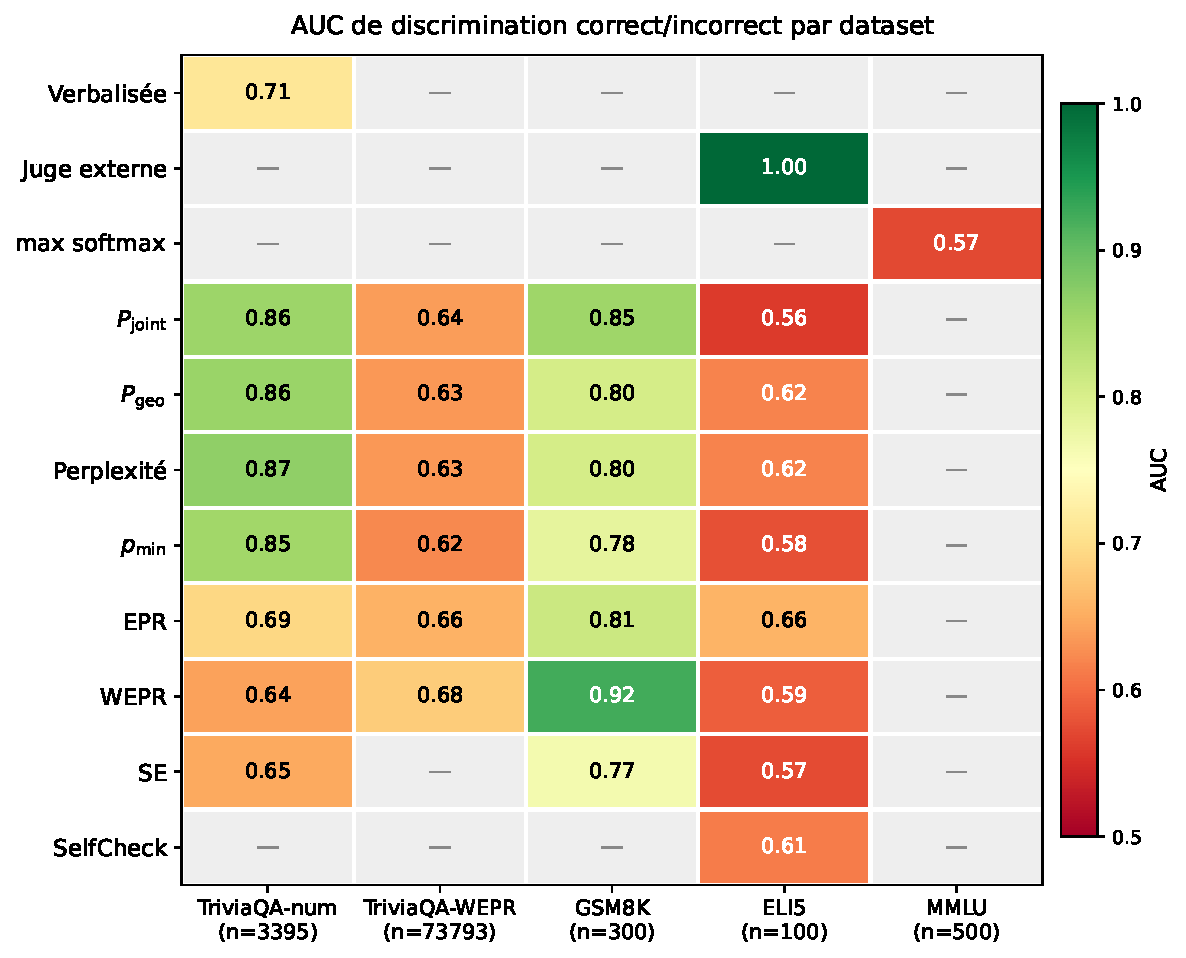
\includegraphics[width=0.95\textwidth]{figures/cross_auc_heatmap.pdf}
\caption{AUC de discrimination correct/incorrect, scores~$\times$~datasets.
Les cellules grises (---) signalent que le score n'est pas applicable
au dataset (absence de distribution top-K, ou score sans signification
hors du cadre considéré). La cellule "Juge externe" sur ELI5 vaut
$1{,}00$ par construction (le score est défini comme la note du juge,
qui sert aussi de cible)~; elle n'est pas interprétable.}
\label{fig:cross_heatmap}
\end{figure}

\paragraph{Trois lectures.}
Premièrement, la hiérarchie des scores n'est pas universelle. Sur les
réponses très courtes de TriviaQA-num (~$\sim 4$~tokens), les
log-probabilités simples (perplexité, $P_{\mathrm{joint}}$,
$P_{\mathrm{geo}}$) atteignent des AUC supérieures à~$0{,}85$, tandis
que WEPR n'atteint que~$0{,}64$. À l'inverse, sur les générations
Chain-of-Thought de GSM8K (~$\sim 188$~tokens), c'est WEPR qui domine
nettement (~$0{,}92$ contre $0{,}80$ pour la perplexité). La règle
qualitative qui s'en dégage est que \emph{le bénéfice marginal d'un
score à pondération apprise comme WEPR croît avec la longueur des
générations}. Inversement, sur des séquences très courtes, la
distribution top-K est trop concentrée pour que la pondération apprise
améliore quoi que ce soit~: les coefficients de WEPR-TriviaQA, calibrés
sur des séquences d'environ~20~tokens, ne sont plus optimaux pour des
réponses de quatre tokens.

Deuxièmement, le score~$P_{\mathrm{joint}}$ chute de
$0{,}857$ sur TriviaQA-num à~$0{,}638$ sur TriviaQA-WEPR, alors qu'il
s'agit du même dataset sous-jacent. La différence vient du
filtre~: TriviaQA-num ne conserve que les questions à réponse numérique
(quelques tokens), tandis que TriviaQA-WEPR conserve toutes les
réponses (textuelles, plus longues). La probabilité jointe perd donc
beaucoup de son pouvoir discriminant dès que la séquence dépasse
quelques tokens, du seul fait que le produit~$\prod_t p_t$ s'écrase
mécaniquement vers zéro. Ce phénomène n'apparaît dans aucune section
prise isolément.

Troisièmement, ELI5 et MMLU ressortent comme les deux régimes les plus
difficiles. Sur ELI5 (réponses longues à jugement humain subjectif),
aucun score ne dépasse~$0{,}66$. Sur MMLU (QCM à quatre options), la
probabilité maximale du choix sélectionné atteint seulement~$0{,}57$
— ce qui ne signifie pas que le modèle ne sait rien, mais que la plage
de softmax sur quatre options est intrinsèquement comprimée et que
cette compression masque une partie du signal d'incertitude.

\paragraph{Et sur la calibration ?}
Le tableau~\ref{tab:cross_ece} reporte l'\emph{Expected Calibration Error}
des scores interprétables comme des probabilités. WEPR atteint sur
TriviaQA-WEPR une ECE de~$0{,}009$ — c'est-à-dire une calibration
quasi parfaite. Cette qualité tient à ce que WEPR sort directement la
probabilité d'une régression logistique optimisée par entropie croisée,
contrairement aux scores bruts (probabilité jointe, perplexité) qui
n'ont aucune raison d'être calibrés en tant qu'estimation de
$\mathbb{P}(\text{correct})$. Sur les générations longues de GSM8K,
$P_{\mathrm{joint}}$ atteint en revanche une ECE de~$0{,}97$~: le
produit des probabilités sur~188~tokens donne une valeur tellement
proche de zéro qu'elle perd tout sens d'estimation calibrée. Cela
constitue un argument fort pour ne plus utiliser~$P_{\mathrm{joint}}$
en tant que probabilité interprétable au-delà de quelques tokens — un
point qui n'apparaissait pas explicitement dans la
section~\ref{sec:generations_longues}.

\begin{table}[H]
\centering
\caption{ECE (10 bins) des scores interprétables comme probabilités sur les
différents datasets.}
\label{tab:cross_ece}
\begin{tabular}{lcccc}
\toprule
Score & TriviaQA-num & TriviaQA-WEPR & GSM8K & ELI5 \\
\midrule
$P_{\mathrm{joint}}$  & 0{,}096 & 0{,}384 & 0{,}969 & 0{,}820 \\
$P_{\mathrm{geo}}$    & 0{,}103 & 0{,}074 & 0{,}082 & 0{,}063 \\
$p_{\min}$            & 0{,}097 & 0{,}297 & 0{,}862 & 0{,}524 \\
WEPR                  & 0{,}030 & \textbf{0{,}009} & 0{,}245 & 0{,}687 \\
Confiance verbalisée  & 0{,}077 & ---     & ---     & ---     \\
\bottomrule
\end{tabular}
\end{table}

\subsection{Synthèse}
\label{sec:transverse_synthese}

La mise en relation des trois sections d'études individuelles permet de
dégager trois constats que ces sections, prises isolément, ne peuvent
pas formuler. Premièrement, \emph{aucun score d'incertitude n'est
universellement supérieur}~: la perplexité domine sur les réponses
courtes ($\mathrm{AUC} \simeq 0{,}87$ sur TriviaQA-num), WEPR domine
sur les générations longues ($\mathrm{AUC} \simeq 0{,}92$ sur GSM8K),
et tous deux échouent sur ELI5 où aucun score ne dépasse~$0{,}66$.
Le choix d'un score doit donc être adapté au régime de génération
considéré (longueur, contrainte syntaxique, présence ou non d'une
vérité terrain numérique).

Deuxièmement, \emph{WEPR généralise mieux qu'on ne le voyait dans la
section~\ref{sec:wepr}}. Le bénéfice de~+2{,}6~points d'AUC observé sur
TriviaQA-WEPR devient~+12~points sur GSM8K, et la version entraînée sur
TriviaQA se transfère telle quelle à GSM8K avec une AUC de~$0{,}79$.
Cela suggère que les coefficients appris par WEPR sur un grand corpus
diversifié encodent une signature d'instabilité \emph{générique} des
LLMs, et qu'ils peuvent servir de détecteur prêt à l'emploi sur un
dataset adjacent. Inversement, WEPR appris sur un petit corpus
fortement déséquilibré (le cas de GSM8K) sur-ajuste la structure des
quelques erreurs disponibles et ne se transfère plus.

Troisièmement, \emph{l'entropie sémantique et les log-probabilités
internes mesurent des aspects complémentaires de l'incertitude}. La
première capture l'instabilité entre échantillons indépendants, les
secondes la concentration locale du modèle sur sa propre génération.
Aucun des deux signaux n'est strictement dominé par l'autre~; un
classifieur qui les combinerait pourrait, en principe, hériter des
forces des deux. Cette piste de combinaison constitue une extension
naturelle pour des travaux futurs.

% =============================================================================
% Fin de la section transverse.
% =============================================================================
